\documentclass[a4paper,14pt]{extarticle}

\usepackage[a4paper,top=20mm,bottom=20mm,left=30mm,right=10mm]{geometry}
\usepackage[T1,T2A]{fontenc}
\usepackage[utf8]{inputenc}
\usepackage[russian]{babel}
\usepackage{indentfirst}
\usepackage{titlesec}
\usepackage{graphicx}
\usepackage{verbatim}
\usepackage{fancyvrb}

\renewcommand{\baselinestretch}{1.3}

\titleformat{\section}{\normalsize\bfseries}{\thesection}{1em}{}
\titleformat{\subsection}{\normalsize\bfseries}{\thesubsection}{1em}{}

\setlength{\parindent}{12.5mm}

\begin{document}

\newpage\thispagestyle{empty}
\begin{center}
    \MakeUppercase{
        Министерство науки и высшего образования Российской Федерации\\
        Федеральное государственное бюджетное образовательное учреждение высшего образования\\
        <<Вятский Государственный Университет>>\\
    }
    Институт математики и информационных систем\\
    Факультет автоматики и вычислительной техники\\
    Кафедра электронных вычислительных машин
\end{center}
\vfill

\begin{center}
    Отчет по лабораторной работе\\
    по дисциплине\\
    <<Алгоритмы и структуры данных>>\\
\end{center}
\vfill

\noindent
\begin{tabular}{ll}
    Выполнили студенты гр. ИВТб-2301-05-00 \hspace{5mm} & \rule[-1mm]{25mm}{0.10mm}\,/Елпашев С.А./  \\
                                                        & \rule[-1mm]{25mm}{0.10mm}\,/Макаров С.А./  \\
    Руководитель преподаватель                          & \rule[-1mm]{25mm}{0.10mm}\,/Пахарева И.В./ \\
\end{tabular}

\vfill
\begin{center}
    Киров 2026
\end{center}

\newpage
\section*{\hspace{12.5mm}Цель работы}
Цель лабораторной работы: разработать бота для игры в шахматы, используя дебютную теорию и алгоритмы с неполным и полным перебором для игры в основной части и эндшпиле.

\section*{\hspace{12.5mm}Задание}
\begin{enumerate}
    \item Разработать алгоритм для игры в дебюте. Алгоритм должен использовать хорошо проработанную шахматную дебютную теорию.
    \item Разработать алгоритм для игры в основной части, когда дебютный алгоритм больше не может продолжать совершать ходы исходя из дебютной теории.
    \item Разработать алгоритм для для игры в эндшпиле.
\end{enumerate}

\section*{\hspace{12.5mm}Решение}
Бот реализован на языке Python в виде консольного приложения, работающего через стандартные потоки ввода-вывода.

Для игры в дебюте используется книга, содержащая набор заранее заготовленных дебютов. На первом ходе бот выбирает случайную дебютную линию, чей первый ход легален. Следующий ход продолжает выбранную линию. Если ожидаемый ход линии нелегален, бот ищет другую линию, у которой уже сделанные ходы совпадают. Если подходящей линии нет, бот переходит к алгоритму поиска лучшего хода.

Рассмотрим работу бота в дебюте на примере итальянской партии, отображенной на рисунке 1. Рисунок имеет следующие обозначения: 1 -- пешка, 2 -- конь, 3 -- слон, 4 -- ладья, 5 -- ферзь, 6 -- король.
=
\pagebreak
\begin{figure}[h]
    \centering
    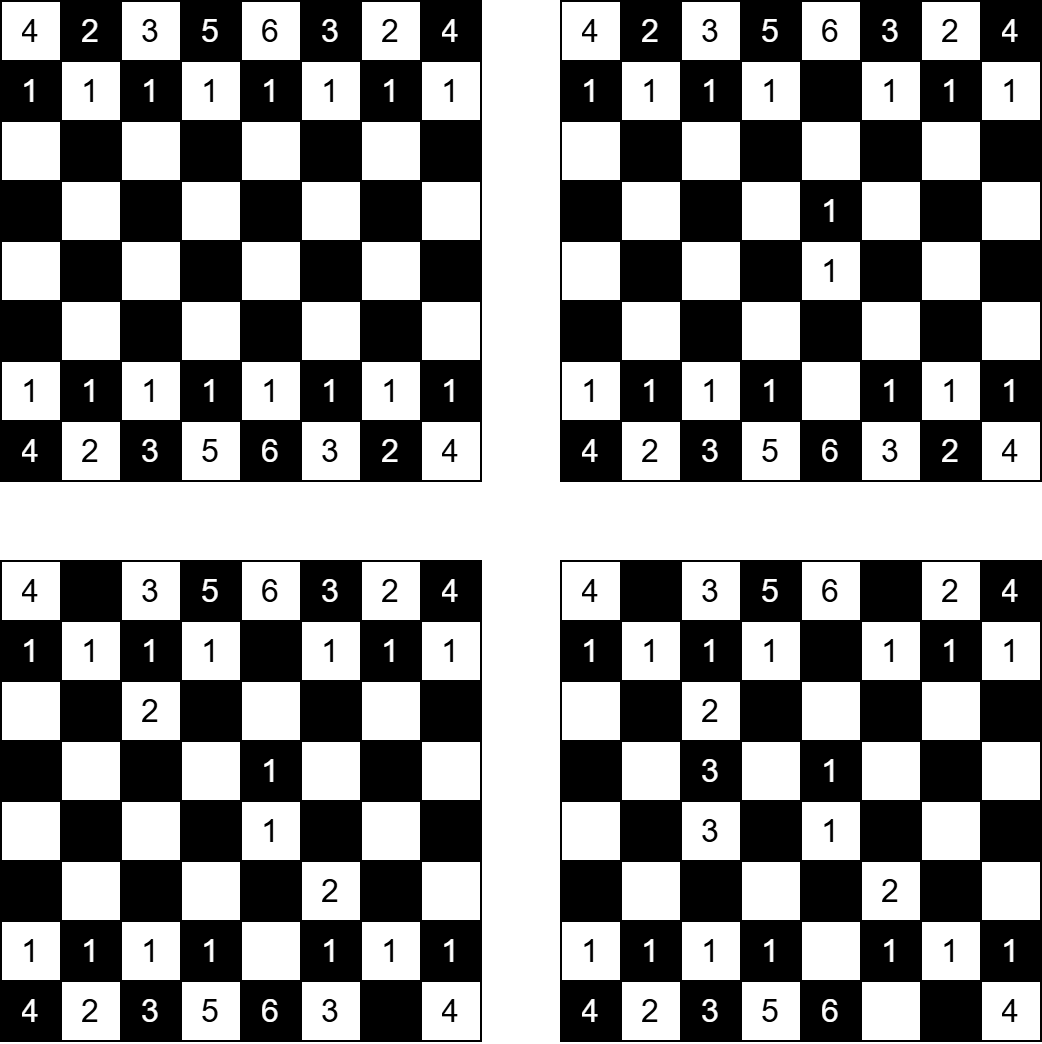
\includegraphics[width=1\linewidth]{img/chess.png}
\end{figure}
\begin{center}
    Рисунок 1 – Ходы итальянской партии
\end{center}

В данном случае сторона белых из списка выбрала итальянскаю партию из книги. В этом случае сторона черных начала искать данный ход в заготовленных дебютах, и после ее определения бот черных начал ходить в соответсвии с ней. После окончания ходов в выбранном дебюте боты переходят к поиску лучшего хода.

Поиск лучшего хода строится на основе оценочной функции, используя методы <<Minimax>> и <<Alpha-beta>>. Она складывает набор числовых признаков. Знак оценки определяется следующим образом:
\begin{itemize}
    \item[--] Очки > 0 -- лучше для бота;
    \item[--] Очки < 0 -- лучше для соперника;
    \item[--] Очки = 0 -- прмерно равная позиция.
\end{itemize}

Одним из факторов оценки является вес фигур. Так как слон в открытых позициях считаются чуть сильнее коня, поэтому слон оценен в 310 против 300 у коня. Это заставляет бота при прочих равных условиях сохранять слонов.
\begin{itemize}
    \item[--] Пешка -- 100;
    \item[--] Конь -- 300;
    \item[--] Слон -- 310;
    \item[--] Ладья -- 500;
    \item[--] Ферзь -- 900;
    \item[--] Король -- 20000.
\end{itemize}

Также для оценки учитывается позиция фигуры. Для каждой фигуры существуют две таблицы 8x8 (для миттельшпиля и эндшпиля), где каждому полю присвоен бонус или штраф:
\begin{itemize}
    \item[--] Кони получают бонусы в центре и штрафы на краях доски;
    \item[--] Слоны и Ферзь получают бонусы за нахождение на центральных полях, откуда они покрывают больше пространства;
    \item[--] Король в начале игры получает огромные штрафы за выход в центр (стимул к рокировке/безопасности), а в конце игры получает бонусы за выход на центральные позиции.
\end{itemize}

Оценочная функция расчитывает сумму $S$ материальных и позиционных факторов, взвешенных относительно фазы игры:

$$S = \frac{S_{mg} * phase + S_{eg} * (256 - phase)}{256}$$

Где:
\begin{itemize}
    \item[--] $S_{mg}$ -- оценка миттельшпиля;
    \item[--] $S_{eg}$ -- оценка эндшпиля;
    \item[--] $phase$ -- коэффициент, означающий фазу игры. 256 -- Миттельшпиль, что означает наличие большого количества фигур, 0 -- фигур осталось мало.
\end{itemize}

Еще одной состовляющей оценки является пешечная структура. Бот анализирует:
\begin{itemize}
    \item[--] Сдвоенные пешки -- штраф, так как они ограничивают друг друга и создают слабости;
    \item[--] Изолированные пешки -- штраф, так как их не могут защитить другие пешки.;
    \item[--] Проходные пешки -- большой бонус. Чем ближе пешка к полю превращения, тем выше бонус. В эндшпиле ценность проходной пешки дополнительно возрастает.
\end{itemize}

Также для оценки хода введены специализированные эвристики.
\begin{itemize}
    \item[--] Безопасность короля -- бот проверяет 6 полей перед королем. Наличие своих пешек там дает бонус. Если количество пешек становиться оценка падает;
    \item[--] Активность ладей -- бонус за открытые линии, большой бонус за 7-ую горизонталь, где ладья атакует пешки соперника и ограничивает короля;
    \item[--] Пара слонов -- если у бота два слона, он получает бонус , так как вместе они контролируют поля обоих цветов;
    \item[--] В миттельшпиле фигуры получают дополнительные очки за контроль «малого центра».
\end{itemize}

Итоговая оценка, возвращаемая функцией выглядит следующим образом:
\begin{itemize}
    \item[--] Положительное -- бот считает, что у него преимущество;
    \item[--] Отрицательное -- бот считает, что позиция хуже;
    \item[--] Около нуля -- Позиция равная.
\end{itemize}

Рассмотрим поэтапно работу бота на визуализаторе в виде веб-версии. На рисунке 2 представлен этап окончания дебюта, так как закончились ходы в предопределенной книге.
\begin{figure}[h]
    \centering
    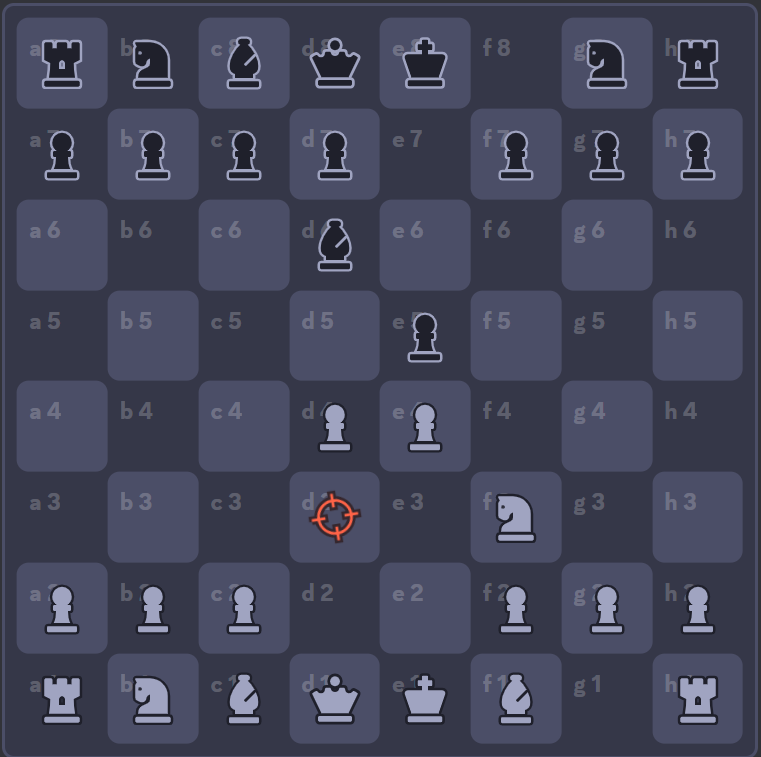
\includegraphics[width=1\linewidth]{img/early.png}\\
    Рисунок 2 – Окончание стадии дебюта
\end{figure}

Далее бот переходит в стадию миттельшпиля. Данный этап игры представлен на рисунке 3.

\begin{figure}[h]
    \centering
    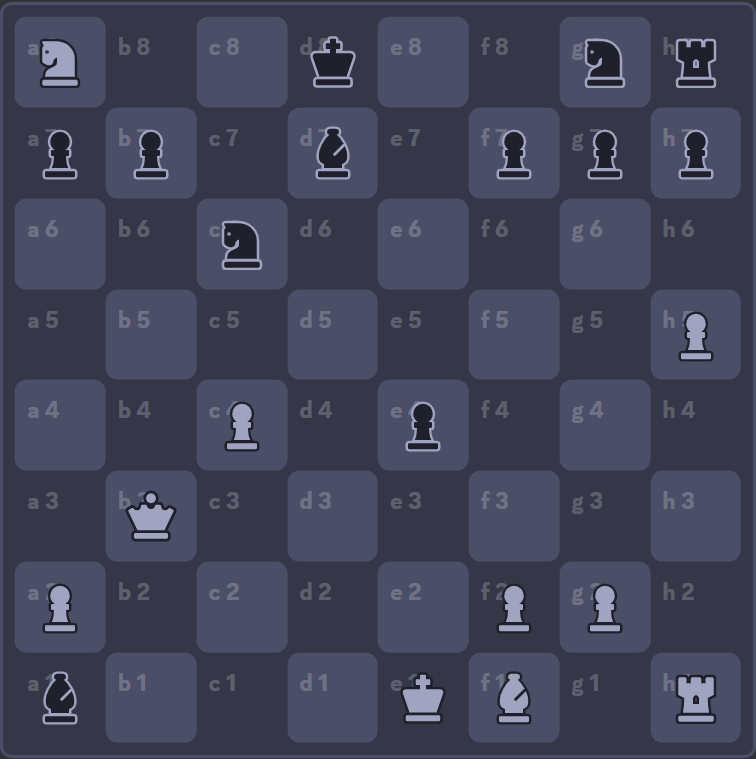
\includegraphics[width=1\linewidth]{img/mid.png}\\
    Рисунок 3 – Миттельшпиль
\end{figure}

После окончания миттельшпиля бот переходит в эндшпиль. Данный этап игры представлен на рисунке 4.

\pagebreak
\begin{figure}[h]
    \centering
    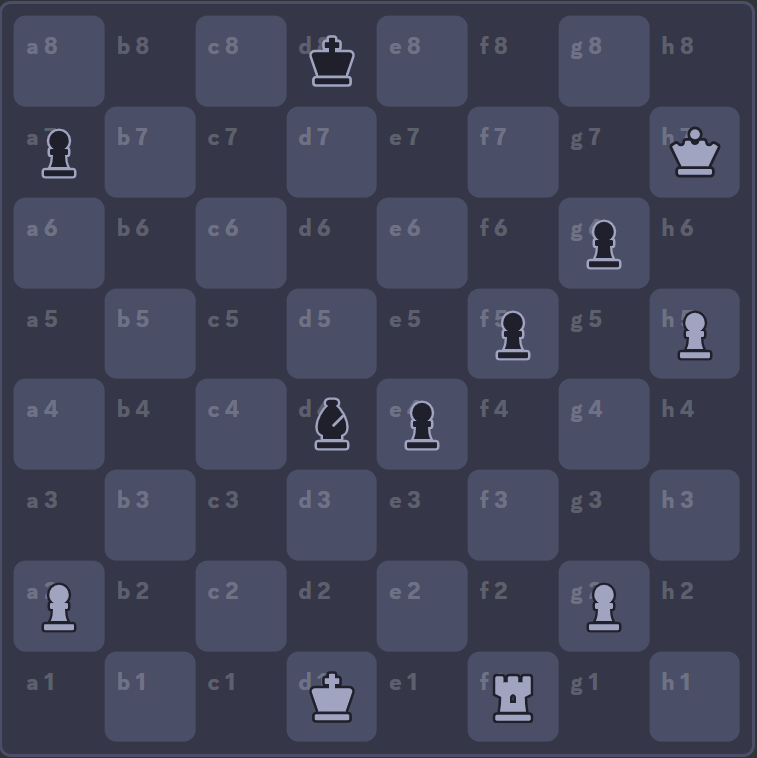
\includegraphics[width=1\linewidth]{img/late.png}\\
    Рисунок 4 – Эндшпиль
\end{figure}

В итоге окончания игры бот, играя за белую сторону выиграл, поставив мат черным. Результат представлен на рисунке 5.

\pagebreak
\begin{figure}[h]
    \centering
    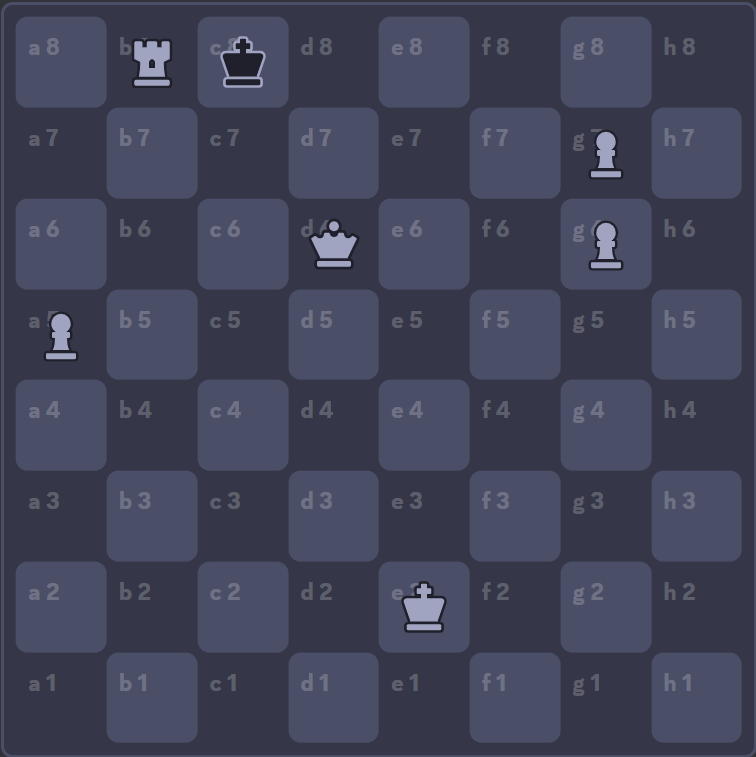
\includegraphics[width=1\linewidth]{img/end.png}\\
    Рисунок 5 – Поставленный мат
\end{figure}

\section*{\hspace{12.5mm}Вывод}
В ходе лабораторной работы был разработан шахматный бот, сочетающий в себе дебютну. книгу и методы численного поиска, такие как <<Minimax>> и <<Alpha-beta>>. Реализованная система позволила боту динамически менять стратегию поведения: в начале игры приоритет отдается безопасности короля и контролю центра, а в эндшпиле — активности короля и продвижению проходных пешек.

\end{document}